\newpage
\subsection[Positionsbestimmung und Funktionsweise]{Positionsbestimmung und Funktionsweise
 \\ \textnormal{\small{\textit {Verfasst von Patrick Senneka}}}}


In diesem Kapitel wird zunächst einmal geklärt, was Positionsbestimmung ist. 
Nach Alex Küpper ist die Positionsbestimmung wie folgt definiert:

\begin{table}[h]
	\centering
	\begin{tabular}{|p{16cm}|}\hline
		\textbf{Zitat 2.1:} \glqq Positioning is a process to obtain the spatial position of a target \grqq  \cite[S.121]{Kuepper2005} \\ \hline
		\textbf{Übersetzung:} Positionsbestimmung ist ein Prozess, um die räumliche Position eines Ziels zu erhalten. \\ \hline
	\end{tabular}
\end{table}

Mit räumlicher Position ist hierbei ein Standort gemeint, der zu einem geeigneten Bezugssystem bestimmt wird. Das bedeutet ein Position die sich auf das Bezugssystem „Weltkarte“ bezieht repräsentiert den geografischen Standort auf der Weltkarte. Die Position mit dem Bezugssystem eines bestimmten Gebäudes repräsentiert den Standort in dem Gebäude. Bsp.: Stockwerk 1 Raum 139b in der DHBW-Mannheim.

Ein weiteres Zitat bezüglich der Positionsbestimmung grenzt den Begriff Positionsbestimmung deutlich von Ortung ab. Dieser Unterschied soll hier auch aufgezeigt werden. Hierzu das Zitat der Webseite www.itwissen.info:

\begin{table}[h]
	\centering
	\begin{tabular}{|p{16cm}|}\hline
		\textbf{Zitat 2.2:} \glqq Die Begriffe Positionsbestimmung und Ortung werden häufig synonym benutzt; sie unterscheiden sich allerdings im Detail. So wird mit der Positionsbestimmung der Ort von Objekten oder Personen eindeutig in einem geografischen Koordinatensystem festgelegt. Sie bildet die Basis für die Ortung und wird dann zur Ortung, wenn Dritten die ermittelte Position mitgeteilt wird. \grqq  \cite[Positionsbestimmung]{itwissen} \\ \hline
	\end{tabular}
\end{table}

Das Zitat ist aussagekräftig und grenzt Positionsbestimmung und Ortung eindeutig voneinander ab.

In diesem Kapitel wird, wie es der Titel vorgibt, nur die Positionsbestimmung betrachtet. Dieser ist die Voraussetzung, um Ortung
%(die Übertragung der Position) 
überhaupt durchzuführen. Allerdings wird im weiteren Teil dieser Arbeit verstärkt die Ortung betrachtet werden. Die Übertragung der Position spielt nämlich zur Bereitstellung eines location-based Services in nahezu allen Fällen eine große Rolle. Da die Positionsbestimmung für die Ortung benötigt wird, diese hier im Detail vorgestellt. 


Bei einer Positionsbestimmung werden Messdaten gesammelt, um die eigenen Position festzulegen. Die Messdaten beziehen sich dabei immer auf festgelegte Fixpunkte, von welchen die Position schon bekannt ist.  Diese Daten sind zum Beispiel Winkel, Geschwindigkeit und Entfernung.

In den kommenden Kapiteln werden unterschiedliche Methoden und Techniken zur Positionsbestimmung vorgestellt. Diese werden in drei Kategorien eingeordnet, die satellitengestützte Positionierung, Positionierung in Mobilfunknetzen und Positionsbestimmung in Gebäuden.
Abbildung \ref{fig:Positionsbestimmung} gibt für die drei Kategorien einen Überblick.

\begin{figure}[h]
\centering
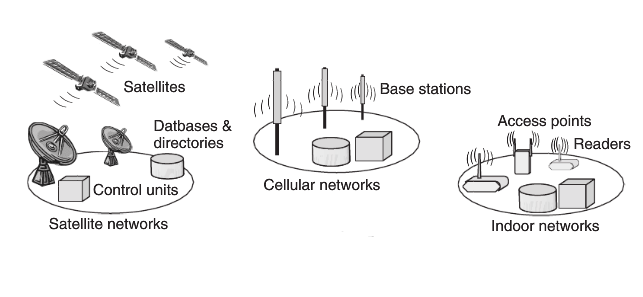
\includegraphics[width=0.99\textwidth]{ref/images/Positionsbestimmung.PNG}
\caption[Infrastruktur zur Positionsbestimmung]{Infrastruktur zur Positionsbestimmung}
\label{fig:Positionsbestimmung}
\cite[S. 124]{Kuepper2005}
\end{figure}

\subsubsection[Kriterien für die Positionsbestimmung]{Kriterien für die Positionsbestimmung
 \\ \textnormal{\small{\textit {Verfasst von Patrick Senneka}}}}

Kein Verfahren zur Positionsbestimmung ist perfekt. 
Deshalb werden die unterschiedlichen Methoden und Techniken zur Positionsbestimmung anhand von drei Qualitäts-Kriterien betrachtet. Diese werden hier kurz erläutert.

\begin{enumerate}
\item Bereich (Scope)\\
Ein Positionssystem ist immer auf einen Bereich bezogen, in dem eine Position theoretisch bestimmt werden kann. Dieser Bereich kann stark, von einem Raum bis zu einem weltweiten Bereich, variieren.\\
$\longrightarrow$ Ein großer Scope ist besser
\item Abdeckung (Coverage)\\
Die Abdeckung eines Positionssystems kann maximal so groß sein, wie es der Bereich zulässt. Die Abdeckung ist die Teilmenge des Bereichs, in dem tatsächlich die Position bestimmt werden kann. So ist es beispielsweise bei einem Satellitenpositionssystem nicht möglich eine Abdeckung in Gebäuden oder unter der Erde zu gewährleisten.\\
$\longrightarrow$ Eine große Abdeckung ist besser
\item Präzision (Precision)\\
Ein Positionssystem kann einen Standort nicht exakt, sondern mit einer gewissen Abweichung bestimmen. Diese Abweichung kann von Umwelteinflüssen abhängen und für eine Positionsbestimmung an der selben Stelle abweichende Ergebnisse liefern. Die Robustheit eines Positionssystem trägt somit auch zur Präzision bei. \\
$\longrightarrow$ Eine höhere Präzision ist besser
\end{enumerate}
\cite[S.183]{Schiller2004}


\subsubsection[Satellitengestützte Positionierung]{Satellitengestützte Positionierung
 \\ \textnormal{\small{\textit {Verfasst von Patrick Senneka}}}}

Satellitengestützte Positionierung basiert, wie der Name schon vermuten lässt, auf Satelliten. 

Das bekannteste System zur satellitengestützte Positionierung ist das Global Positioning System, dass mit GPS abgekürzt wird. Auf GPS wird nach einer Erläuterung über das generelle Funktionsprinzip von Satellitenpositionierung eingegangen.

Eine Grundvoraussetzung für Satellitengestützte Positionierung sind Satelliten, die sich in der Erdumlaufbahn befinden und elektromagnetische Wellen auf die Erde funken. Damit eine Position auf der Erdoberfläche mit Hilfe von Satelliten errechnet/bestimmt werden kann, muss auch ein Gerät vorhanden sein, dass die elektromagnetischen Wellen der Satelliten empfangen und verarbeiten kann.

Ist das gegeben kann prinzipiell die Position des Nutzers auf der Erdoberfläche anhand von der exakten Position von mindestens drei Satelliten ($s_{n}$) und des Abstands zu diesen Satelliten ($r_{m}$) bestimmt werden.

\cite[S. 188]{Schiller2004}

%Vergleiche hierzu Abbildung \ref{fig:Grundprinzip Satelliten}

\begin{figure}[h]
\centering
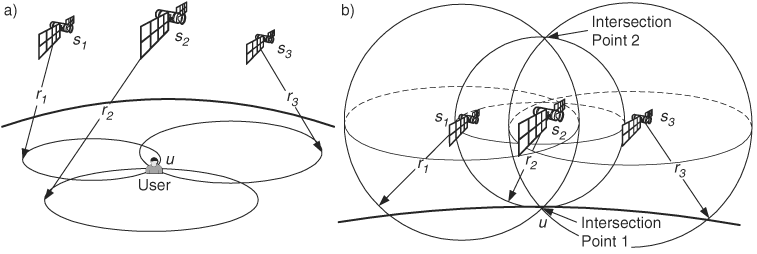
\includegraphics[width=0.99\textwidth]{ref/images/prinzip_satelliten.png}
\caption[Grundprinzip Satelliten Positionsbestimmung]{Grundprinzip Satelliten Positionsbestimmung}
\label{fig:Grundprinzip Satelliten}
\cite[S. 188]{Schiller2004}
\end{figure}

In Abbildung \ref{fig:Grundprinzip Satelliten} a) stellen die Kreise Positionen auf der Erde dar, an denen eine User-Position anhand des gemessenen Abstands ($r_{m}$) möglich ist. In dieser Darstellung mit drei Satelliten ist die User-Position eindeutig an dem Schnittpunkt aller drei Kreise. 
In Abbildung \ref{fig:Grundprinzip Satelliten} b) wird die Darstellung ins dreidimensionale überführt. Hierbei ist nun zu erkennen, dass die Kreise zu Kugeln geworden sind. Daraus resultierend gibt es nun einen zweiten Schnittpunkt. Für die Positionsbestimmung gibt es nun zwei mögliche User-Positionen. Dieses Problem beseitigt man einfach, indem man die logisch wahrscheinlichere Position als richtige ansieht. In der Abbildung wäre das Intersection Point 1, da Intersection Point 2 im Weltall liegt und davon auszugehen ist, dass sich Menschen auf der Erdoberfläche befinden.
\cite[S. 188]{Schiller2004}

Es wurde nun erläutert, wie sich die Position ermitteln lässt, wenn dem Nutzer die Position der Satelliten und der Abstand zu diesen bekannt ist. Wie diese Werte ermittelt werden, wurde noch nicht erwähnt. Darauf wird nun eingegangen.

\textbf{Satelliten Positionen:}\\
Satelliten kreisen um die Erde. Sie sind also Ständig in Bewegung. 

\begin{figure}[h]
\centering
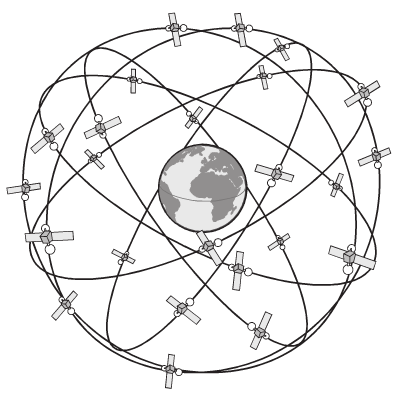
\includegraphics[width=0.4\textwidth]{ref/images/GPS_Umlaufbahn.PNG}
\caption[Umlaufbahn von GPS Satelliten]{Umlaufbahn von GPS Satelliten}
\label{fig:Umlaufbahn Satelliten}
\cite[S. 164]{Kuepper2005}
\end{figure}

Da sie in zuvor festgelegten Umlaufbahnen kreisen, kann die Position eines Satelliten abhängig von der Zeit errechnet werden. 
Diese Berechnung kann ohne Probleme auf einem Smartphone stattfinden. Die einzigen Daten die dazu nötig sind, ist eine aktuelle Uhrzeit, sowie die Satellitennamen mit der dazugehörigen Umlaufbahn. Solche Daten befinden sich standardmäßig auf GPS fähigen Geräten. Bei Bedarf, durch den Ausfall oder das Hinzukommen neuer Satelliten, werden diese Daten aktualisiert.
\cite[S. 189]{Schiller2004}


\textbf{Abstand zu den Satelliten:}\\
Der Abstand zu Satelliten wird anhand der Zeit berechnet, die das Signal vom Satelliten bis zum Empfänger benötigt. Diese Zeit wird dadurch ermittelt, dass vom Satelliten die aktuelle Zeit gesendet wird. Sobald diese beim Empfänger ankommt wird der Zeitunterschied $ \bigtriangleup t $ zur aktuellen Zeit ermittelt. Da sich elektromagnetische Wellen mit Lichtgeschwindigkeit $ c $ fortbewegen, beträgt die Geschwindigkeit näherungsweise 300.000 $km/s$. Mit der Formel $ r = c \bigtriangleup t$ lässt sich dann die Entfernung zum Satelliten ermitteln. Das Verfahren funktioniert allerdings nur, wenn die Uhren vom Satelliten und des Empfängers exakt synchronisiert sind. 
\cite[S. 189]{Schiller2004}

Eine Abweichung der Uhren von nur $1\mu s$ ergibt aufgrund der hohen Geschwindigkeit der elektromagnetischen Wellen eine Abweichung der bestimmten Position von ca. 300 Metern.
\cite[S. 189]{Schiller2004}

Diese Aussage verdeutlicht, wie wichtig es ist die Uhren exakt zu synchronisieren. Deshalb wird nun ein Verfahren zu Synchronisation von Uhren vorgestellt.


\textbf{Verfahren zur Uhren Synchronisation:}

Jeder Satellit ist mit einer Atomuhr ausgestattet um immer die richtige Zeit zu senden. Eine Atomuhr in ein Smartphone einzubauen macht allein schon aus wirtschaftlicher Sicht keinen Sinn. Deshalb muss es ein Verfahren geben, mit dem die Uhren synchronisiert werden könne, oder der Unterschied zwischen den Uhren bestimmt werden kann.
\cite[S.189]{Schiller2004}

Das Grundprinzip dieses Verfahrens wird nun erläutert. Dazu werden zunächst einige Variablen definiert.

$ t_{s} $ steht für die Systemzeit des Satelliten, an der das Signal gesendet wurde.

$ \tilde{t}_{s = t_{s} + \delta t_{s}} $ ist die Zeit des Satelliten unter Berücksichtigung der Abweichung $ \delta t_{s} $ zur exakten Zeit.

$ t_{u} $ steht für die Systemzeit der Users, zu der er das Signal empfangen hat.

Die Systemzeit des Users kann eine Abweichung zur exakten Zeit haben. Deshalb wird für die weitere Betrachtung $ \tilde{t}_{u = t_{u} + \delta t_{u}} $ unter Berücksichtigung der Abweichung $ \delta t_{u} $ zur exakten Zeit verwendet.

$ \bigtriangleup \tilde{t} = \tilde{t}_{u} - \title{t}_{s} $ ist die gemessene Zeit zwischen dem Abschicken des Signals vom Satelliten bis zum Empfang des Signals beim User.

$ c $ gibt die Lichtgeschwindigkeit an.

Im Abschnitt \glqq Abstand zu den Satelliten \grqq wurde schon die Formel zur Berechnung des Abstands $ r = c \bigtriangleup t $ erwähnt. Diese basiert allerdings darauf, dass beide Uhren synchronisiert sind.

Hier wir diese Formel dahingehend angepasst, dass die Abweichungen $\bigtriangleup t$ von den Systemzeiten berücksichtigt werden. Das ist dann der gemessen Abstand $p$:

\grqq \cite[S. 189 - 190]{Schiller2004}

\glqq 
\begin{align}
p &= c * \bigtriangleup \tilde{t} \\
  &= c * (\tilde{t}_{u} - \tilde{t}_{s}) \\
  &= c * ((t_{u} + \delta t_{u}) - (t_{s} + \delta t_{s})) \\
  &= c * (t_{u} - t_{s}) + c * (\delta t_{u} - \delta t_{s}) \\
  &= r + c * (\delta t_{u} - \delta t_{s})
\end{align}
\grqq \cite[S. 190]{Schiller2004}

Die Systemzeit des Satelliten ist bei dieser Betrachtung als exakt anzusehen, da Satelliten mit einer Atomuhr ausgestattet sind und von Bodenstationen kontrolliert werden. $\delta t_{s}$ ist damit als 0 anzusehen.

Daraus erhalten wir $p = r + c * \delta t_{u}$

$r$ kann hierbei durch die Koordinaten des Satelliten und des Users dargestellt werden: $p = \sqrt{(s_{x} - u_{x})^{2} + (s_{y} - u_{y})^{2} + (s_{z}-u_{z})^{2}} + c * \delta t_{u}$

Diese Gleichung enthält nun vier unbekannte Variablen $u_{x}, u_{y}, u_{z}$ und $\delta t_{u}$. 

Um diese Gleichung zu lösen benötigt man diese vier unbekannten Variablen. Jeder dieser Variable kann selbst wieder über eine Gleichung bestimmt werden. Um alle vier Gleichungen zu lösen sind dann vier Satelliten nötig. 

Es gibt nun mehrere Möglichkeiten diese Lösung anzugehen. Es kann zum Beispiel durch ein Näherungsverfahren geschehen. Herr Schiller verweist in deiner Arbeit dabei auf die Möglichkeit eine Taylor Reihe.

Da es ab dieser Stelle nur noch eine mathematische Aufgabe ist die Lösung zu finden, und es dafür wiederum unterschiedliche Ansätze gibt, wird darauf nicht weiter eingegangen.

\cite[S. 190]{Schiller2004}


\textbf{GPS}

Das Global Position System wurde vom Amerikanischen Verteidigungsministerium entwickelt. Es gibt eine Variante, die nur dem Militär zugänglich ist und eine, die der Zivilbevölkerung frei zur Verfügung steht. 

Das GPS System besteht auf 24 Satelliten, die um die Erde kreisen. Die Satelliten können über Basisstationen, die auf der ganzen Erde verteilt sind, ihre Uhren synchronisieren und ihre richtige Umlaufbahn beibehalten. 
\cite[S. 162]{Kuepper2005}


\begin{figure}[h]
\centering
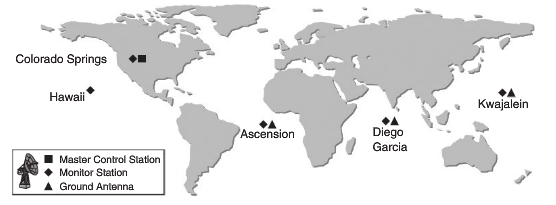
\includegraphics[width=0.99\textwidth]{ref/images/GPS_Basisstation.PNG}
\caption[GPS Basissationen]{GPS Basissationen}
\label{fig:GPS Basissationen}
\cite[S. 163]{Kuepper2005}
\end{figure}

Das GPS basiert grundsätzlich auf den zuvor vorgestellten Mechanismen zur Standortbestimmung. 

Es gibt allerdings einen Unterschied in der militärischen und der zivilen Variante. Die militärische Variante bietet eine höhere Präzision, steht allerdings nur Ländern die der NATO angehören zur Verfügung. 

Die zivile Variante bietet im Normalfall eine fast so hohe Präzision, wie die militärische, kann aber von der U.S. Army durch einen Mechanismus, der Selective Avaulability (SA) heißt deutlich ungenauer gemacht werden.

\cite[S. 194 - 196]{Schiller2004}

Vergleiche hierzu Abbildung \ref{fig:GPS Praezision}.

PPS steht für die militärische Variante wohingegen SPS für die zivile Variante des GPS steht.

\begin{figure}[h]
\centering
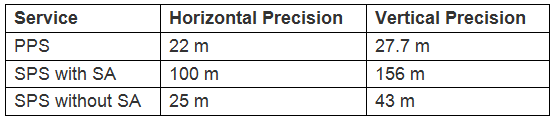
\includegraphics[width=0.6\textwidth]{ref/images/GPS_Praezision.PNG}
\caption[GPS Präzision]{GPS Präzision}
\label{fig:GPS Praezision}
\cite[S. 195]{Schiller2004}
\end{figure}

Die Präzision von GPS kann durch Differential GPS nochmals verbessert werden. Dazu wird in einer Basisstation, zu der eine exakte Position vorhanden ist, die GPS Position ermittelt. Gibt es Abweichungen durch die Atmosphäre wird von der Basistation eine Korrektur erstellt, die dann an den User weitergeleitet werden kann, um auch dessen Präzision zu verbessern.
\cite[S. 196]{Schiller2004}

Vergleiche hierzu Abbildung \ref{fig:DGPS}
\begin{figure}[h]
\centering
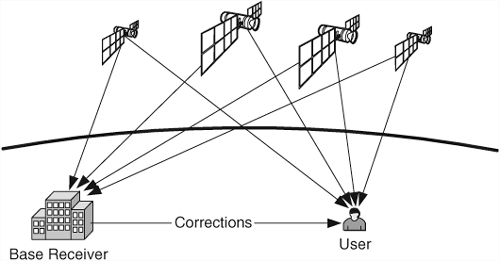
\includegraphics[width=0.99\textwidth]{ref/images/DGPS.PNG}
\caption[Präzision Differential GPS]{Präzision Differential GPS}
\label{fig:DGPS}
\cite[S. 196]{Schiller2004}
\end{figure}

Betrachtet man Satelliten Positionierung und im speziellen GPS kann man für die Qualitätskriterien die folgende Bewertung abgeben.

$\longrightarrow$ Bereich (Scope) Prinzipiell ist eine Standortbestimmung auf der ganzen Welt möglich.

$\longrightarrow$ Abdeckung (Coverage) Die Position kann überall auf der Erdoberfläche, mit einer Ausnahme, der Positionsbestimmung in Gebäuden, bestimmt werden. Das bietet eine sehr große Abdeckung.

$\longrightarrow$ Präzision (Precision) Eine hohe Präzision wird durch viele Satelliten und Korrektursignale ermöglicht. Die Position ist so  robust gegen Umwelteinflüsse.

\cite[S. 187]{Schiller2004}

Die Kosten zum Betreiben von Satelliten sind immens hoch. Es gibt allerdings auch andere Positionierungssysteme, die auf schon vorhandene Funknetze setzen. Diese werden nun vorgestellt.

\subsubsection[Positionierung in (Mobil)Funknetzen]{Positionierung in (Mobil)Funknetzen
 \\ \textnormal{\small{\textit {Verfasst von Patrick Senneka}}}}

Ein weit verbreitetes Funknetz ist das Mobilfunknetz. Es ist in über 190 Ländern verfügbar.\cite[206]{Schiller2004} Um zu verdeutlichen, wie groß die Abdeckung in Deutschland ist, wird die Netzabdeckung von drei großen Mobilfunkanbietern aufgezeigt. Vergleiche hierzu Abbildung \ref{fig:GSM}.

\begin{figure}[h]
\centering
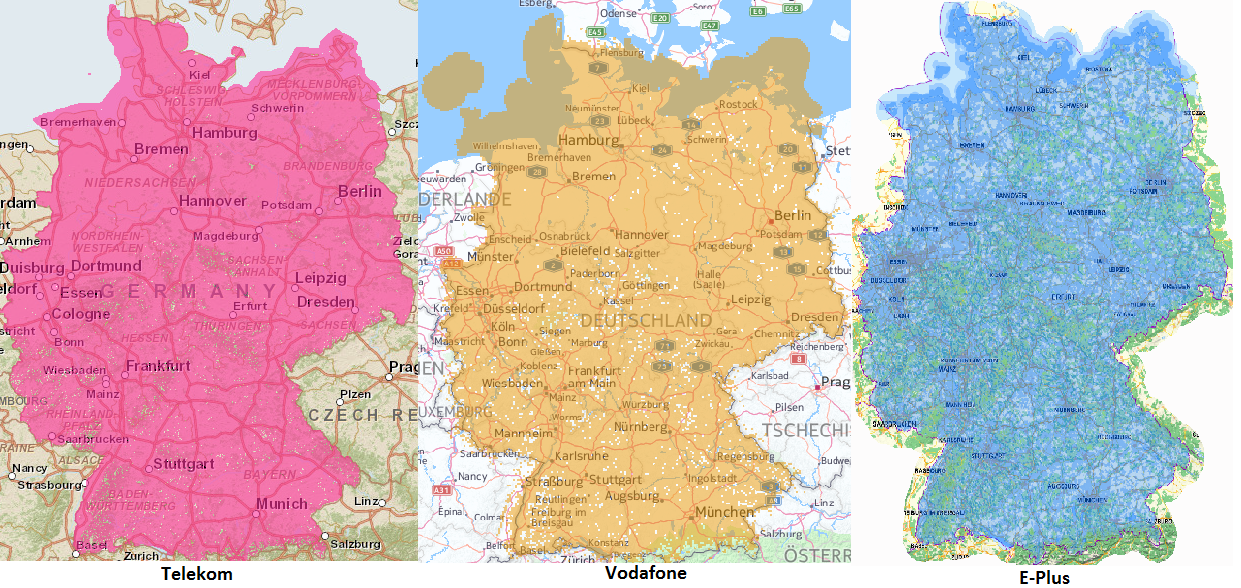
\includegraphics[width=0.99\textwidth]{ref/images/GSM.PNG}
\caption[GSM Abdeckung in Deutschland]{GSM Abdeckung in Deutschland}
\label{fig:GSM}
\cite{Telekom} \cite{Vodafone} \cite{Eplus}
\end{figure}

Die Abbildungen zeigen eine nahezu vollständige Abdeckung Deutschlands durch das GSM Netz. Partiell ist je nach Netzbetreiber die Abdeckung durch GSM nicht gegeben.

Zu Abbildung \ref{fig:GSM} ist noch anzumerken, dass es sich hierbei um Darstellungen der einzelnen Mobilfunkanbietern handelt. Es ist davon auszugehen, dass auf Grund von Marketingeinflüssen auf die Grafiken eine höhere Abdeckung dargestellt wird, als in der Realität vorhanden ist. Um einen groben Eindruck für die Abdeckung in Deutschland zu bekomme, sollten diese Abbildungen dennoch ausreichend sein.


Basierend auf GSM gibt es verschieden präzise Ansätze die Position eines Netzers über dessen Handy zu finden.


Der technisch einfachste aber auch unpräziseste Ansatz ist die Positionsbestimmung anhand des Funkmasten, an dem des Handy angemeldet ist. Das Prinzip dahinter ist, dass sich ein Handy immer mit dem stärksten Signal eines Funkmasten verbindet. Von dem Funkmast mit dem stärksten Signal ist auszugehen, dass es der nächstgelegene ist. Die Position, sowie ein Radius, in dem dessen Signal empfangen werden kann ist dem Betreiber eines jedem Funkmasten bekannt. 

Sobald sich ein Handy mit einem Funkmasten verbindet, wird das in einer dezentralen Datenbank (Visitor Location Register) erfasst. Die Informationen aus der VLR Datenbank werden anschließend in die zentrale Datenbank des Betreibers des Funkmasten, dem Home Location Register, übertragen. Der Betreiber kann anhand seiner Positionsinformationen des Funkmasten ermitteln, in welchem Bereich die Position des Handys bzw. des Nutzers ist. Vergleiche Abbildung \ref{fig:CoO}.

\cite[S. 207]{Schiller2004}

\begin{figure}[h]
\centering
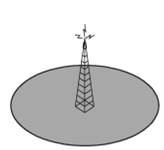
\includegraphics[width=0.2\textwidth]{ref/images/CellOfOrigin.PNG}
\caption[Cell of Origin]{Cell of Origin}
\label{fig:CoO}
\cite[S. 209]{Schiller2004}
\end{figure}

Die Präzision dieser Positionierung hängt von der Größe der Funkzelle ab. So ist in Städten von einem Radius von ca. 1 km auszugehen, wohingegen in ländlicheren Regionen der Radius einer Funkzelle bis zu 35 km betragen kann.
\cite[S. 207]{Schiller2004}


Ein präziseres Verfahren wurde von der Firma Ericsson entwickelt und heißt Mobile Positioning System (MPS). 
\cite[S. 207 - 208]{Schiller2004}

Dieses Verfahren besteht aus mehreren Teilverfahren, die hier nacheinander vorgestellt werden.

\begin{enumerate}
\item Cell of Global Identity \\
Dieses Verfahren entspricht den zuvor beschriebenen Positionsbestimmung anhand der Funkzelle. Vergleiche Abbildung \ref{fig:CoO}. Diese Variante des MPS bildet die Grundlage für alle weiteren.
\item Segment antennas \\
Eine Funkzelle breitet sich meist $360^{o}$ um einen Funkmasten aus. Dieser Bereich kann nicht von einer Antenne abdeckt werden. Dafür werden normalerweise drei bis vier Antennen benötigt. Jede einzelne Antenne ist dann für einen geringeren Winkel zuständig ($90^{o}$ oder $120^{o}$).

Die Position eines Handys kann anhand der genutzten Antenne auf ein Segment der Funkzelle eingeschränkt werden.
\cite[S. 208]{Schiller2004}

Vergleich hierzu Abbildung \ref{fig:SA}.

\begin{figure}[h]
\centering
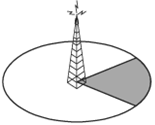
\includegraphics[width=0.2\textwidth]{ref/images/SegmentAntennas.PNG}
\caption[Antennen Segment]{Antennen Segment}
\label{fig:SA}
\cite[S. 209]{Schiller2004}
\end{figure}

\item Timing Advance \\
In einer Funkzelle gibt es mehr als ein Gerät. Deshalb gibt es ein \glqq Time-division multiplexing \grqq , was jedem Gerät einen Zeitslot gibt, in dem es mit der Funkzelle kommunizieren kann. Dieses Verfahren berücksichtigt auch die Laufzeit des Signals von einem Handy zu einem Funkmasten. Die Informationen über die Laufzeit des Signals können dazu verwendet werden die Entfernung des Geräts zu einem Funkmasten zu bestimmen. Die Entfernung kann dabei in Abstufungen von ca. 555 Metern ermittelt werden. Unter Zuhilfenahme des Segment antenna Verfahrens kann die Präzision der Position so weiter verbessert werden.
\cite[S. 208]{Schiller2004}

Vergleiche hierzu Abbildung \ref{fig:TA}.

\begin{figure}[h]
\centering
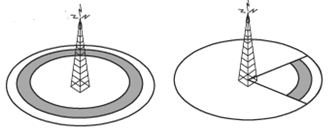
\includegraphics[width=0.4\textwidth]{ref/images/TimingAdvance.PNG}
\caption[Timing Advance mit Segment antenna]{Timing Advance mit Segment antenna}
\label{fig:TA}
\cite[S. 209]{Schiller2004}
\end{figure}

\item Uplink Time of Arrival \\
Befindet sich ein Handy in mindestens 4 Funknetzen kann zu allen verfügbaren Funknetzen nach dem \glqq Timing Advance \grqq Verfahren die Entfernung bestimmt werden. 

Ähnlich wie bei der Satelliten Positionierung ist es dann möglich eine genaue Position zu ermitteln. Diese ist dann auf 50 - 150 Meter genau.
\cite[S. 209]{Schiller2004}

Vergleiche Abbildung \ref{fig:Up}.

\begin{figure}[h]
\centering
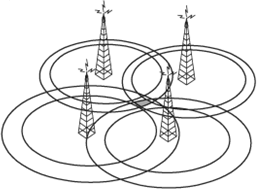
\includegraphics[width=0.2\textwidth]{ref/images/Uplink.PNG}
\caption[Uplink Time of Arrival]{Uplink Time of Arrival}
\label{fig:Up}
\cite[S. 209]{Schiller2004}
\end{figure}

\end{enumerate}


$\longrightarrow$ Bereich (Scope) Die Standortbestimmung ist in 190 Ländern möglich. 

$\longrightarrow$ Abdeckung (Coverage) Die Abdeckung der Funknetze ist in den Ländern sehr hoch. Es ist sogar möglich in Gebäuden den Standort zu bestimmen.

$\longrightarrow$ Präzision (Precision) Die Präzision liegt im besten Fall bei 50 - 150 Metern, was für viele LBS schon ausreichend sein dürfte.




\subsubsection[Positionsbestimmung in Gebäuden]{Positionsbestimmung in Gebäuden
 \\ \textnormal{\small{\textit {Verfasst von Patrick Senneka}}}}

Systeme zur Positionsbestimmung in Gebäuden haben eine vergleichsweise geringe Abdeckung. Sie bieten sich besonders für den Einsatz in Gebäuden an, da diese eine Geringe Fläche haben und  da dort Verfahren wie GPS versagen. 

Auf zwei Verfahren, die Positionsbestimmung in Gebäuden wird nun im genauer eingegangen. Zuerst wird die Positionsbestimmung anhand von WLAN Netzwerken dargestellt. Danach werden Radio Beacons genauer betrachtet.

\textbf{WLAN Netzwerke}\\
Heutzutage sind in vielen Gebäuden WLAN-Netzwerke verfügbar. Ein gutes Beispiel dazu ist die DBHW-Mannheim. Dort ist in nahezu jedem Raum ein WLAN Accesspoint vorhanden.

Von Microsoft gibt es ein prototypisches Verfahren, welches anhand der Signalstärke aller verfügbaren WLAN Accespoints eine Positionierung in WLAN-Netzwerken ermöglicht. 

Das Verfahren basiert darauf, dass man Messpunkte erstellt. Zu den erstellten Messpunkten ist die Position bekannt. Aus vielen Messpunkten ergibt sich dann eine Tabelle.

\cite[S. 210]{Schiller2004}

Eine solche Tabelle sieht nach Herr Schillers Buch Location-based Services so aus:

\begin{figure}[h]
\centering
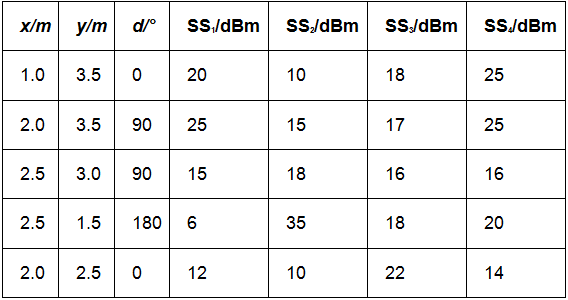
\includegraphics[width=0.7\textwidth]{ref/images/WLAN_Tabelle.PNG}
\caption[WLAN Messwerttabelle]{WLAN Messwerttabelle}
\cite[S. 210]{Schiller2004}
\end{figure}

Anhand solch einer Tabelle kann zur Positionierung die Signalstärke der einzelnen WLAN Accesspoints ermittelt werden und auf den am besten passenden Standort gemappt werden. So ist eine Positionierung in einem zuvor festgelegtem Raster möglich.

Das Problem an dem Verfahren ist, dass wenn zu wenig Accespoints vorhanden sind, wird die Position schnell ungenau. Außerdem sind Messungen zum Konfigurieren erforderlich. 

Ein alternativer Ansatz wäre Triangulation. Das ist ähnlich zum dem Verfahren, das bei GPS vorgestellt wurde. Der Abstand zu den Accesspoint kann anhand er Signalstärke errechnet werden. Die Position von den Accesspoint ändert sich nicht und ist bekannt. Damit kann aus dem Schnittpunkt der Radium am die Accesspoints der eigene Standort ermittelt werden.

\cite[S. 209-211]{Schiller2004}

$\longrightarrow$ Bereich (Scope) Die Reichweite eines WLAN Accesspoint beträgt maximal 100 Meter. In Deutschland und anderen Ländern ist WLAN nicht flächendeckend Verfügbar, sondern nur in wenigen Städten vorhanden. Der Bereich ist meist auf ein Gebäude beschränkt.

$\longrightarrow$ Abdeckung (Coverage) Die Abdeckung von WLAN Netzwerken entspricht ziemlich genau dem Scope. 

$\longrightarrow$ Präzision (Precision) Die Präzision von WLAN Positionierung ist bis auf wenige Meter genau. Damit ist eine hohe Präzision gegeben.

\textbf{Radio Beacons} \label{sec:radio}

Radio Beacons sind kleine Geräte, die ständig elektromagnetische Wellen senden. Diese übermitteln Daten, wie die ID des Radio Beacons, bis zu einer Entfernung von 30 Metern.

Alleine durch die Lokalisation eines Beacons (Funkzelle) ist eine hohe Genauigkeit gegeben. Beacons können so konfiguriert werden, dass ihr Signal nur in einem Radius von ca. 5 Meter empfangen werden kann. Ermittelt ein Gerät (Handy) solch einen Beacon ist die eigene Position schon sehr präzise bestimmt.

Auch bei dieser Technologie ist es wieder möglich Signale von mehreren Beacons zur Positionsbestimmung zu verwenden. Dadurch wird die ermittelte Position genauer. Bei Beacons ist es sogar möglich eine 3D-Position zu ermitteln.

Ähnlich zu dem bei Satelliten Positionsbestimmung beschriebenem Verfahren ist es auch hier wieder möglich eine genaue Position zu ermitteln, wenn man Signale von mehreren Beacons empfängt. Das Verfahren beruht auf einer Abstandsmessung anhand der Time of Arrival von Signalen. Ein beispielhaftes Verfahren dafür heißt SpotOn.
Nutz man SpotOn wird eine Präzision der Position von 3 Meter erreicht. Das ist ein sehr gutes Wert.

\cite[S. 201 - 204]{Schiller2004}

Vergleiche Abbildung \ref{fig:SpotOn}.

\begin{figure}[h]
\centering
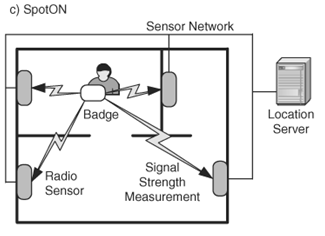
\includegraphics[width=0.5\textwidth]{ref/images/SpotOn.PNG}
\caption[SpotOn]{SpotOn}
\label{fig:SpotOn}
\cite[S. 201]{Schiller2004}
\end{figure}


$\longrightarrow$ Bereich (Scope) Der Bereich kommt auf die Anzahl der Beacons an, ist aber als klein einzustufen.

$\longrightarrow$ Abdeckung (Coverage) Die Abdeckung in dem gegebenen Scope sollte 100 prozentig sein.

$\longrightarrow$ Präzision (Precision) Die Präzision ist mit 3 Metern sehr gut. 






\subsubsection[Kombination von Verfahren zur Positionsbestimmung]{Kombination von Verfahren zur Positionsbestimmung
 \\ \textnormal{\small{\textit {Verfasst von Patrick Senneka}}}}

Jedes der zuvor vorgestellten Verfahren hat Vor- und Nachteile, die hauptsächlich in der Präzision und der Abdeckung liegen.
Mit Smartphones ist es möglich all die vorgestellten Verfahren zu nutzen, da diese fast immer mit GPS, WLAN und Bluetooth, sowie immer mit Mobilfunk ausgestattet sind.
Bei diesen Möglichkeiten ist es naheliegend, dass man eine Kombination der Verfahren zur Positionsbestimmung verwendet, um stets die präziseste Position zu ermitteln. 

Bei Cordova/Phonegap werden zur präzisen Positionsbestimmung die Verfahren GPS, IP, RFID, WLAN und GSM eingesetzt. \cite{phonegap2015}
Die Verfahren laufen parallel, so dass jedes eine Position ermittelt und die Präzision dieser liefert. Der präziseste Standort wird dann für die App verwendet.